\documentclass[12pt]{article}
\usepackage{gensymb}
\usepackage{amsmath}
\usepackage{graphics}
\usepackage{graphicx}
\graphicspath{{storage/self/primary/Download/asgnt1/fig}}
\providecommand{\brak}[1]{\ensuremath{\left(#1\right)}}
\providecommand{\myvec}[1]{\ensuremath{\begin{pmatrix}#1\end{pmatrix}}}
\begin{document}
\title{\textbf{ASSIGNMENT-11.10.4.9}}
\date{}
\maketitle
\textbf{Question :} Find the value of $p$ so that the three lines $3x+y-2=0,px+2y-3=0$ and $2x-y-3=0$ may intersect at one point.


\textbf{Solution :}
\begin{align}  
&\myvec{
    3 &1&-2 \\
     $p$&2&-3\\
     2&-1&-3
}\\
\xrightarrow[R_2'=2R_2-3R_1]{R_3'=R_3-R_2}&\myvec{
    3&1&-2\\
     $2p-9$&1&0\\
     2-p&-3&0}\\
 \xrightarrow{R_3''=R_3+3R_2}&\myvec{
    3&1&-2\\
     $2p-9$&1&0\\
     5p-25&0&0}\\
\end{align}
For getting the determinant zero the last row must be zero .

So,
\begin{align}
    5p-25&=0\\
    p&=5
\end{align}

\begin{figure}
    \centering
    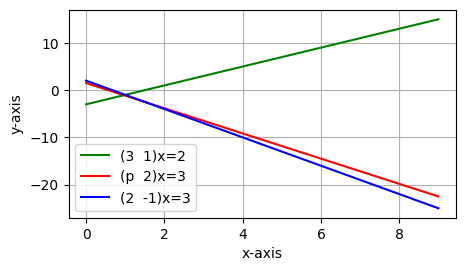
\includegraphics[width=\columnwidth]{fig/11.10.4.9.png}
    \caption{}
    \label{11.10.4.9}
\end{figure}
\end{document}

